%%%%%%%%%%%%%%%%%%%%%%%%%%%%%%%%%%%%%%%%%%%%%%%%%%%%%%%%%%%%%%%%%%%%%%%%%%%%
% AGUtmpl.tex: this template file is for articles formatted with LaTeX2e,
% Modified March 2013
%
% This template includes commands and instructions
% given in the order necessary to produce a final output that will
% satisfy AGU requirements.
%
% PLEASE DO NOT USE YOUR OWN MACROS
% DO NOT USE \newcommand, \renewcommand, or \def.
%
% FOR FIGURES, DO NOT USE \psfrag or \subfigure.
%
%%%%%%%%%%%%%%%%%%%%%%%%%%%%%%%%%%%%%%%%%%%%%%%%%%%%%%%%%%%%%%%%%%%%%%%%%%%%
%
% All questions should be e-mailed to latex@agu.org.
%
%%%%%%%%%%%%%%%%%%%%%%%%%%%%%%%%%%%%%%%%%%%%%%%%%%%%%%%%%%%%%%%%%%%%%%%%%%%%
%
% Step 1: Set the \documentclass
%
% There are two options for article format: two column (default)
% and draft.
%
% PLEASE USE THE DRAFT OPTION TO SUBMIT YOUR PAPERS.
% The draft option produces double spaced output.
%
% Choose the journal abbreviation for the journal you are
% submitting to:

% jgrga JOURNAL OF GEOPHYSICAL RESEARCH
% gbc   GLOBAL BIOCHEMICAL CYCLES
% grl   GEOPHYSICAL RESEARCH LETTERS
% pal   PALEOCEANOGRAPHY
% ras   RADIO SCIENCE
% rog   REVIEWS OF GEOPHYSICS
% tec   TECTONICS
% wrr   WATER RESOURCES RESEARCH
% gc    GEOCHEMISTRY, GEOPHYSICS, GEOSYSTEMS
% sw    SPACE WEATHER
% ms    JAMES
% ef    EARTH'S FUTURE
%
%
%
% (If you are submitting to a journal other than jgrga,
% substitute the initials of the journal for "jgrga" below.)

\documentclass[jgrga, draft]{agutex}
% \documentclass[jgrga]{agutex}
% To create numbered lines:

% If you don't already have lineno.sty, you can download it from
% http://www.ctan.org/tex-archive/macros/latex/contrib/ednotes/
% (or search the internet for lineno.sty ctan), available at TeX Archive Network (CTAN).
% Take care that you always use the latest version.

% To activate the commands, uncomment \usepackage{lineno}
% and \linenumbers*[1]command, below:

\usepackage{lineno}
\linenumbers*[1]

%  To add line numbers to lines with equations:
%  \begin{linenomath*}
%  \begin{equation}
%  \end{equation}
%  \end{linenomath*}
%%%%%%%%%%%%%%%%%%%%%%%%%%%%%%%%%%%%%%%%%%%%%%%%%%%%%%%%%%%%%%%%%%%%%%%%%
% Figures and Tables
%
%
% DO NOT USE \psfrag or \subfigure commands.
%
%  Figures and tables should be placed AT THE END OF THE ARTICLE,
%  after the references.
%
%  Uncomment the following command to include .eps files
 % \usepackage[pdflatex]{graphicx}
 \usepackage{graphicx}
 \DeclareGraphicsExtensions{.pdf, .png, .jpg, .eps}
 \graphicspath{ {./figs/} }

%
%  Uncomment the following command to allow illustrations to print
%   when using Draft:
 \setkeys{Gin}{draft=false}
%
% Substitute one of the following for [dvips] above
% if you are using a different driver program and want to
% proof your illustrations on your machine:
%
% [xdvi], [dvipdf], [dvipsone], [dviwindo], [emtex], [dviwin],
% [pctexps],  [pctexwin],  [pctexhp],  [pctex32], [truetex], [tcidvi],
% [oztex], [textures]
%
% See how to enter figures and tables at the end of the article, after
% references.
%
%% ------------------------------------------------------------------------ %%
%
%  ENTER PREAMBLE
%
%% ------------------------------------------------------------------------ %%

% Author names in capital letters:
\authorrunninghead{HAMMAN ET AL.}

% Shorter version of title entered in capital letters:
\titlerunninghead{LAND-OCEAN COUPLING IN RASM}

%Corresponding author mailing address and e-mail address:
\authoraddr{Corresponding author: Bart Nijssen,
Department of Civil \& Environmental Engineering, Box 352700,
University of Washington, Seattle, WA 98195-2700, USA.
(nijssen@uw.edu)}

\begin{document}

%% ------------------------------------------------------------------------ %%
%
%  TITLE
%
%% ------------------------------------------------------------------------ %%


\title{Land-Ocean Coupling in the Regional Arctic System Model}

%% ------------------------------------------------------------------------ %%
%
%  AUTHORS AND AFFILIATIONS
%
%% ------------------------------------------------------------------------ %%


% Use \author{\altaffilmark{}} and \altaffiltext{}

% \altaffilmark will produce footnote;
% matching \altaffiltext will appear at bottom of page.

\authors{Joseph Hamman,\altaffilmark{1}
Bart Nijssen,\altaffilmark{1},
Anthony Craig,\altaffilmark{2}
Wieslaw Maslowski\altaffilmark{2},
Robert Osinski\altaffilmark{3},
and Andrew Roberts\altaffilmark{2}}

\altaffiltext{1}{Department of Civil \& Environmental Engineering,
University of Washington, Seattle, WA, USA.}
\altaffiltext{2}{Department of Oceanography, Naval Postgraduate School,
Monterey, CA, USA.}
\altaffiltext{3}{Polish Institute of Oceanology, Sopot, Poland.}


%% ------------------------------------------------------------------------ %%
%
%  ABSTRACT
%
%% ------------------------------------------------------------------------ %%

% >> Do NOT include any \begin...\end commands within
% >> the body of the abstract.

\begin{abstract}
The purpose of the abstract is twofold: (1) state the nature of the investigation and (2) summarize the important conclusions of this investigation. The abstract should be suitable for separate publication in an abstract journal and be adequate for indexing. Make sure to check for the following:

It is set as a single paragraph.
It is limited to 250 words for all journals except GRL where the limit is 150 words.
It does not include table or figure mentions.
If it has reference citations that are part of the sentence, they should be in roman type and have parentheses around the year; parenthetical reference citations will be deleted.
All abbreviations used in the abstract are defined.
\end{abstract}

%% ------------------------------------------------------------------------ %%
%
%  BEGIN ARTICLE
%
%% ------------------------------------------------------------------------ %%

% The body of the article must start with a \begin{article} command
%
% \end{article} must follow the references section, before the figures
%  and tables.

\begin{article}

%% ------------------------------------------------------------------------ %%
%
%  TEXT
%
%% ------------------------------------------------------------------------ %%

\section{Introduction}

We have implemented a horizontal river routing scheme representing the streamflow flux between the land and ocean model components within the recently developed Regional Arctic System Model [RASM].
In this paper, we introduce the RVIC streamflow routing model and describe its coupling within RASM.
We evaluate the performance of RVIC in fully-coupled RASM simulations, comparing model simulated streamflows to in-situ observations.
We then highlight the role of the streamflow flux in the ocean component in RASM, utilizing a set of sensitivity experiments aimed at understanding the importance of accurately representing streamflow in coupled climate simulations in the Arctic.

Approximately 11\% of the global terrestrial runoff drains into the Arctic Ocean, which holds only 1\% of the Earth's saltwater \citep{Lewis_2000,Lammers_2001}.
Streamflow is the largest contributor of freshwater to the Arctic Ocean and making up approximately 38\% of the total freshwater freshwater flux entering the Arctic Ocean \citep{Serreze_2006}.
During the spring and summer months, the fractional contribution of freshwater to the Arctic from streamflow is much larger.
Across the Arctic region, the annual runoff hydrograph is characterized by a prominent spring freshet, with approximately 60\% of the annual runoff volume occurring between April and July \citep{Lammers_2001}.

The seasonal freshwater flux from the land to the ocean can play an important role in coastal ocean dynamics and hydrography, as well as to sea ice formation and melt \citep{Rabe_2011,Fichot_2013}.
Runoff from Arctic river basins is the primary source of buoyancy-driven currents such as the Alaska, Siberian, Norwegian, and East Greenland coastal currents \citep[e.g.][]{Morison_2000,Boyd_2002,McGeehan_2012}.
Such currents redistribute both fresh water and heat, which locally play important roles in shelf dynamics and shelf-basin interactions.
Another important aspect is the effect of buoyancy delivered by rivers on the onset of sea ice formation in winter and melt in spring/summer [need to cite].
Less salty water freezes at higher temperatures, and therefore does not have to be cooled as much as higher salinity water to freeze.
Thus, for a warming and freshening Arctic, the onset of freezing in areas highly influenced by streamflow may be partially buffered against regional warming.

Long-term river runoff maintains the surface freshwater layer in the Arctic Ocean and is necessary to balance freshwater export through Fram Strait and the Canadian Arctic Archipelago into the North Atlantic [need to cite].
This freshwater layer is also important for maintaining the stratified structure of the Arctic Ocean \citep{Nummelin_2015}.
Although warmer water (less dense) exists at depth in the Arctic Ocean, stratification is maintained by the density differences between the fresh mixed layer and the more saline halocline and Atlantic water layers.
These stratifying processes serves to limit the heat flux into the mixed layer from below.

% [ocean / sea ice specific studies]
The terrestrial freshwater flux has been shown to be an important driver of ice-ocean dynamics in coupled ice-ocean models \citep[e.g.][]{Lique_2015}.
\citet{Newton_2008} applied observed climatological runoff at the largest nine rivers in the Arctic basin and used dye tracers to visualize the spatial distribution of runoff; finding the highest concentrations of river runoff along the Siberian coast.
Despite our understanding of the importance of river runoff in Arctic Ocean dynamics, \citet{Nummelin_2015} show that fully-coupled global climate models [GCMs] poorly represent the vertical structure of the Arctic Ocean, with many models failing to accurately reproduce the observed profiles of temperature and salinity in the upper 500 m.

Numerous observational and modeling studies have explored the seasonal and inter-annual behavior of Arctic runoff.
\citet{Lammers_2001} compiled the R-ArcticNET database, a regional hydrographic record of monthly mean streamflow observations, including over 3,700 streamflow gauges.
R-ArcticNET was used by \citet{Shiklomanov_2009} in their investigation of increasing river discharge in the largest Eurasian rivers and by \citep{Tan_2011} in their investigation of changes in spring snowmelt timing.
\citet{Dai_2009} extended portions of the R-ArcticNET database through 2007 for a smaller collection of coastal streamflow gauges.
\citet{Adam_2007, Adam_2008, Su_2005, Dai_2009} all have used uncoupled land surface models, in conjunction with routing schemes to simulate streamflow across the pan-Arctic region.
These studies have all led to improved understanding of the terrestrial hydroclimate in the Arctic and how the seasonal streamflow dynamics in the Arctic basin respond to changes in climate and water management activities.
However, there has not been significant research applied to understanding the role of streamflow in coupled processes in the Arctic.

% [other climate models that include coupled land-ocean dynamics]
Previous studies have included streamflow routing models within coupled climate models.
Cell-to-cell routing methods, such as the River Transport Model \citep[RTM][]{Branstetter_2003} have been applied globally in a number of GCMs, including in the Community Earth System Model [CESM].
These cell-to-cell models are typically difficult to parameterize across a range of spatial scales \citep{Sushama_2004}.
Source-to-sink routing models, akin to the RVIC model used in this study, have also been previously applied in coupled models \citep[e.g.][]{Olivera_2000}.
Source-to-sink routing methods do not explicitly track streamflow between grid cells, rather they parameterize the distribution and travel time of runoff between a source grid cell and an outlet grid cell.
However, in recent years, the literature has been mostly silent in terms of development of streamflow routing schemes coupled within earth system models.
In fact, \citet{Bring_2015}, in their recent synthesis of CMIP5 runoff dynamics, conclude that a significant community effort should be made to improve the understanding and modeling of basin scale freshwater fluxes in coupled climate modeling.
This notion is further echoed by \citet{Lique_2015} in their review paper of the representation of the Arctic hydrologic cycle in coupled climate models.

In this paper, we describe the land-ocean coupling in the Regional Arctic System Model [RASM, see section~\ref{sec:rasm}].
We introduce the RVIC streamflow routing model and present results from fully-coupled RASM simulations where the land and ocean are coupled via the runoff flux.
The analysis presented here compares simulated streamflow to observations at streamflow gauging locations and explores the role of the terrestrial freshwater flux in the ice-ocean components of the climate system.

\section{Models}

\subsection{RASM}
\label{sec:rasm}

The Regional Arctic System Model [RASM] is a fully coupled, high spatial and high temporal resolution regional earth system model applied over the pan-Arctic domain.
RASM has recently been developed under the support of the Department of Energy Earth System Modeling program.
Principle goals of the modeling project are to better understand the interaction between physical systems in the Arctic drainage basin, to advance understanding of past and present states of Arctic climate, and to improve seasonal to multi-decadal prediction capabilities of key Arctic indicators.
Existing model components, typically run off-line of one another are coupled using the CESM coupled model framework and the CPL7 flux coupler \citep{Craig_2011}.
Below, we provide a brief description of the five component models in RASM version 1.0.
The reader is encouraged to see the cited RASM specific references for more information on the specific implementation of individual component models.
For the purposes of this paper, we are principally concerned with the coastal streamflow flux and its role in the Arctic Ocean system, therefore our description below mainly focuses on the streamflow and ocean model components.

\begin{enumerate}
\item CICE: The Los Alamos Sea Ice model \citep{Hunke_2010} is physically based dynamic sea ice model.
\citet{Roberts_2015b} provide a description of the application of CICE, version 5, within RASM.
\item POP: The Parallel Ocean Program model \citep{Smith_2010} is a general circulation ocean model.
Osinski et al. [Manuscript in Preparation] provide a description of the application of POP, version 2, within RASM.
Of particular relevance to this study, POP uses a virtual salinity flux to represent changes in ocean salinity due to surface fluxes of freshwater (runoff, precipitation, and evaporation).
The virtual salt flux is calculated as
\begin{equation}
     VSF= -F_w S
\end{equation}

where $F_w$ is a sum of the fluxes from streamflow, precipitation, evaporation, and sea ice melting and freezing. $S$ is reference salinity, which is a surface salinity of grid cell where input of fresh water is taking place.

\item VIC: The Variable Infiltration Capacity model \citep{Liang_1996} is a macroscale land surface hydrology model.
\citet{Hamman_2016} provide a description of the application of VIC, version 4, within RASM.
\item WRF: The Weather Research and Forecasting atmospheric model \citep{Skamarock_2007} is a mesoscale meteorological model.
\citet{Cassano_2015} provide a detailed description of the WRF model, version 3.2, as it is applied in RASM.
\item RVIC: The RVIC streamflow routing model is an adapted version of the \citet{Lohmann_1996} linear routing model frequently used to route the runoff flux from the VIC model.
A complete description of the RVIC model is provided in section~\ref{sec:rvic}.
\end{enumerate}

In RASM Version 1.0, the land, atmosphere, and runoff components share a 50-km near-equal-area North Pole stereographic grid mesh.
The ocean and sea ice models share a 1/12$^{\circ}$ rotated stereographic grid mesh.
Models are coupled every 20 minutes in the configuration described by \citet{Roberts_2015a}.

\subsection{RVIC}
\label{sec:rvic}

The RVIC streamflow routing model is a modified version of the routing model typically used to post-process VIC model output \citep{Lohmann_1996, Lohmann_1998a}.
The original \citet{Lohmann_1996} model has been used in many offline modeling studies across spatial scales from 1/16$^{\circ}$ to 2$^{\circ}$ \citep[e.g.][]{Nijssen_1997,Lohmann_1998b,Su_2005}.
RVIC is a source-to-sink model that solves a linearized version of the Saint-Venant equations.
The model has two distinct steps, the preprocessing step where linear time invariant impulse response functions [IRFs] are developed (see sections ~\ref{sec:irfs} and ~\ref{sec:remap}), and a the convolution step where distributed runoff from the land surface model is routed to downstream points (see section~\ref{sec:convolution}).

The RVIC model differs from the original \citet{Lohmann_1996} model in four main ways:

\begin{enumerate}
\item RVIC completely separates the development of the IRFs from the flow convolution step,
\item RVIC allows the development of the IRFs to be done on flow direction grids that do not match that of the land model (see section~\ref{sec:irfs}),
\item The RVIC convolution scheme operates in a space-before-time pattern, facilitating direct coupling with land surface models (see section~\ref{sec:convolution}),
\item RVIC includes numerous infrastructure improvements, including parallel processing, the ability to store the model state, and to read and write netCDF files.
\end{enumerate}

\subsubsection{Impulse response function development}
\label{sec:irfs}

The source-to-sink response of flow from any model grid cell to a downstream point is represented as a linear and time invariant response to an impulse of runoff.
Therefore, the development of the IRF between any source and sink points may be described as a function of the horizontal travel time of water within the source grid cell and to the downstream point with the addition of a flow diffusion parameter.
The horizontal travel distance is computed using a flow direction raster \citep[e.g.][]{Wu_2011}
The Saint-Venant equation

 \begin{equation}
     \frac{\partial Q}{\partial t} = D \frac{\partial^2 Q}{\partial x} + C \frac{\partial Q}{\partial x}
 \end{equation}

represents the flow $Q$, at time $t$, at a downstream point $x$, as a function of the wave velocity, $C$, and the diffusivity, $D$; both of which may be estimated from geographical data.

Eq. (1) can be solved with convolution integrals

 \begin{equation}
	Q(x,t) = \int_0^t U(t-s)h(x,s)ds
 \end{equation}

where

 \begin{equation}
	h(x, t) = \frac{x}{2t\sqrt{\pi tD}}exp\left(-\frac{(Ct-x)^2}{4Dt}\right)
 \end{equation}

is Green’s impulse response function, and $U$ is a unit hydrograph representing the distribution of flow from within each source grid cell to the edge of the source grid cell.
The Saint-Venant equations are solved to determine flow response from every source to outlet pair.

\subsubsection{Upscaling and basin aggregation}
\label{sec:remap}

The development of the impulse response functions may be done on a high resolution (e.g. 1/16$^{\circ}$) flow network such as the one developed by \citet{Wu_2011}.
Whereas the typical employment of the \citet{Lohmann_1996} model requires that the flow direction grid and the land surface model grid match exactly, the RVIC implementation first upscales and aggregates the high resolution IRF grid to the land surface model grid [\ref{fig:2}].
The upscaling process uses the first-order conservative remapping technique developed by \citep{Jones_1999}.
Because the remapping scheme is conservative, the unit response to runoff (unit hydrograph) from each source grid cell is maintained.
Finally, the regridded IRFs are aggregated to include all basins flowing into a single outlet grid cell.

\subsubsection{Convolution}
\label{sec:convolution}

Once the development of the IRFs complete, RVIC performs a simple linear convolution of the IRFs and runoff fluxes from the land model.
In essence, RVIC aggregates the flow contribution from all upstream grid cells at every timestep, distributing them in time according the IRF.

\subsection{Coupling}
\label{sec:coupling}

In nature, turbulent mixing and other diffusive processes combine to gradually spread freshwater along the coast and into the open ocean.
In a coupled modeling environment however, these processes are difficult to represent at the spatial scales that ocean and sea ice models are run at.
To simulate the dispersion of freshwater throughout each ocean grid cell within RASM, a diffusion scheme is applied to avoid unrealistic salinity gradients that would occur when a river’s entire outflow is applied to one ocean grid cell.
The mapping from the runoff grid to the ocean grid is produced as a preprocessing step using the runoff and ocean grids and masks.
Each runoff gridcell is mapped to the nearest ocean grid cell.
The flux is then smoothed over all grid cells in a 300 km radius with distance weighting e-folding scale of 1000 km such that the total quantity is conserved from runoff to ocean.
This smoothing prevents excessively large and unrealistic runoff fluxes into any single ocean grid cell and encourages computational stability within the ocean model while representing the distributed changes in salinity due to the land-ocean freshwater flux.

\subsubsection{RVIC in RASM}

The IRFs used in RASM were developed using the \citet{Wu_2011} 1/16$^{\circ}$ flow direction rasters.
The baseline RASM simulation used a spatially constant flow velocity and diffusion of 0.6 m/s and a 3,000 m$^2$/s, respectively.
These parameters were chosen using the calibration methods described below in section~\ref{sec:parameters}.
IRFs were developed for each of the 95,001 coastal 1/16$^{\circ}$ grid cells bordering the ocean model, and were aggregated and remapped to the 4,841 coastal grid cells on the 50-km near equal area land surface grid.

\subsection{Parameter Selection}
\label{sec:parameters}

A brute force parameter selection procedure was performed to select the velocity and diffusion parameters for the RVIC model applied in RASM.
For this procedure, RVIC was run offline of RASM at a daily timestep and was forced using daily runoff fluxes from the fully coupled RASM simulation described as $RASM_{ERA}$ in \citep{Hamman_2016}.
The velocity parameter was varied between 0.2 and 1.5 m/s and the diffusion was varied between 500 and 4,000 m\textsuperscript{2}/s.
Individual pairs of parameters were evaluated using a modified version of the overlap statistic \citet{Perkins_2012}.
The overlap statistic, which was originally introduced as a measure of likeness for probability density functions, is applied here to the normalized mean monthly hydrographs of the six largest river basins in the RASM model domain [Figure \ref{fig:1}] and the observations from \citet{Dai_2009}.
The overlap statistic is perhaps the best performance measure of the routing model because it focuses entirely on the shape of the hydrograph and does not take into account bias in the flow volume which is determined by the land surface model (See Figure \ref{fig:3}).
The pair of velocity and diffusions parameters, 0.6 m/s and 3,000 m\textsuperscript{2}/s respectively, was chosen to maximize the volume weighted composite overlap statistic for the largest six rivers in the RASM domain (See Figure \ref{fig:4}).

\section{Model Simulations and Data}

In this paper, we present results from two RASM simulations, each using ERA-Interim boundary conditions, $RASM_{CONTROL}$, and $RASM_{NOROF}$ using RASM version 1.0 (Tag R1010).
We also highlight the impact of the calibration procedure with a offline RVIC simulation, $RVIC_{FAST}$, forced with runoff fluxes from $RASM_{CONTROL}$.
All three simulations were run from September 1, 1979 through December 31, 2014, however we use an analysis period of January 1, 1990 and December 31, 2014, allowing for a 10 year model spinnup.
Both RASM simulations began with the same initial states (see \citet{Hamman_2016} for more details) and use the same land, atmosphere, ocean, and sea ice model configurations.
These simulations only differ in the following ways:
\begin{itemize}
     \item $RASM_{CONTROL}$: uses the calibrated RVIC parameters described above.
     \item $RASM_{NOROF}$: does not include the runoff flux from the land to the ocean.
     \item $RVIC_{FAST}$: stand-alone RVIC simulation forced with $RASM_{CONTROL}$.
          This simulation uses velocity and diffusion parameters of 2.0 m/s and 2,000 m\textsuperscript{2}/s.
          These parameters are frequently used as default parameters with the RVIC model and were the original parameters used when evaluating the model.
\end{itemize}

We compare output from RASM simulations to streamflow observations in the \citet{Dai_2009} dataset.
This dataset provides mean monthly streamflow observations at the most downstream gauging location for 42 individual river basins within the RASM domain and analysis period.

\section{Results}

\subsection{Routed Streamflow Hydrographs}

Our analysis of the streamflow hydrograph extends the results of \citet{Hamman_2016} to the monthly timestep.
Figure \ref{fig:5} compares the monthly routed hydrographs for $RASM_{CONTROL}$ and $RVIC_{FAST}$ at the six streamflow gauge locations shown in Figure \ref{fig:3} compared to the observations from \citep{Dai_2009}.
The annual bias, annual overlap, and monthly RMSE statistics for these six monthly hydrographs are shown in Table\ref{table:1}.
The $RASM_{CONTROL}$ hydrographs in the Amur, Lena, and Yukon basins match the observations best, with overlap statistics between X-X.
In the Ob, Yenisey, and Mackenzie River basins, the $RASM_{CONTROL}$ routed streamflow suffers from positive biases in the winter and spring and negative biases in the summer.
Consequently, the overlap statistics for these rivers are lower (X-X).
In these basins, during the winter, it is clear that VIC is under estimating the baseflow flux.
For most of the basins shown in Figure \ref{fig:5}, the timing of the peak month in the $RASM_{CONTROL}$ simulation occurs in the same month as the observations.
The notable exception to this is in the Ob River basin, where the runoff regime is acutely influenced by extensive wetlands and permafrost, and the spring peak occurs a month early (May vs. June).
Compared to the normalized hydrographs in Figure \ref{fig:4}, the majority of the disagreement in Figure \ref{fig:5} is due to the bias in the runoff flux, which is entirely controlled by the land surface model.
\citet{Hamman_2016} provide a more detailed, intermodel comparison of the runoff biases in RASM.

The peak spring freshet in $RVIC_{FAST}$ occurs about one month earlier than in $RASM_{CONTROL}$.
On average, this leads to overlap statistics that are about 15 percent lower than the $RASM_{CONTROL}$ simulation.
The differences in the routing parameters used in the $RASM_{CONTROL}$ and $RVIC_{FAST}$ simulations can be clearly identified in the annual cycle column of Figure \ref{fig:5}.
The bias in timing of the peak spring freshet is mostly due to the difference in streamflow velocity (2.0 vs. 0.6 m/s), whereas the shape of the hydrograph is largely determined by the diffusivity parameter (2000 vs. 6000 m\textsuperscript{2}/s).
[TODO: add bias and nse to timeseries, add overlap statistic to annual cycle or put it all in a table]

Figure \ref{fig:6} shows a Taylor Diagram comparing the RASM simulated hydrographs at 42 observation locations.
The Taylor diagram shows the correlation along the arc and the normalized standard deviation along the radius.
The contours denote lines of equal root-mean-square error (RMSE) where zero is a correlation of 1.0 and a standard deviation of 1.0.
While the correlation coefficients in $RVIC_{FAST}$ are not distributed according to the flow magnitude, the largest basins in $RASM_{CONTROL}$ tend to perform better with correlation coefficients typically increasing by about 0.3.
This is likely due to our choice to calibrate the runoff parameters using only the largest basins in the domain.
While the correlations are shown to improve in all of the basins shown in Figure \ref{fig:6}, the standard deviations are not shown to be significantly impacted by the calibration.
This indicates that the variability in the monthly timeseries in not significantly controlled by the routing model.

\subsection{Role of high resolution coastal streamflow on ocean and sea ice dynamics}
Runoff is a major source of freshwater to the Arctic Ocean (AO). It maintains the vertical stratification and may influence the ocean circulation.
The freshwater content is vital property of AO.
Comparing computational results (fig X and XX) there is a clear example how large the change is in Beaufort Gyre (BG).
The change of runoff influence basin-scale hydrology.
The BG, wind-driven ocean current accumulates freshwater in the Canada Basin.

We begin by exploring the influence of coastal streamflow on the mean surface salinity and temperature across the RASM ocean domain.
We compare the two fully coupled simulations ($RASM_{CONTROL}$ and $RVIC_{FAST}$) and one partially coupled simulation ($RASM_{NOROF}$) to the PHC climatological dataset.
In the control simulation, which has the most realistic streamflow timing, differences in the surface salinity are small...

Observation [cite] and modeling \citep[e.g.][]{Nummelin_2015} based studies have indicated the importance of realistic streamflow fluxes in maintaining the observed stratified temperature and salinity profiles in the Arctic Ocean.
Figure \ref{fig:8} shows the average seasonal ocean basin temperature and salinity profiles for each of the three RASM simulations considered here, compared to the PHC climatology.

\section{Discussion}

\subsection{Impacts on the Arctic Climate System}
The largest and most direct impact that the inclusion of the streamflow flux has within the Arctic climate system is on near coastal surface salinity in the ocean.
We have shown that the fully coupled $RASM_{CONTROL}$ simulation better represents the upper ocean salinity than the $RASM_{NOROF}$ or $RASM-HCASE$...

\subsection{Routing Processes}
The RVIC model is a source-to-sink linear routing model that uses time-invariant IRFs to route streamflow to coastal grid cells in RASM.
While we have shown that RVIC, coupled within RASM, is able to capture the first order behavior of streamflow processes effecting the position and shape of the annual hydrograph, we know it lacks mechanisms to accurately capture many of the second order processes unique to the Arctic.
For example, there is no mechanism in the RVIC model to account for non-linear routing processes such as overbank flow, wetlands, ice jams, reservoir operations, and industrial or agricultural withdrawals.
\citet{Adam_2007} highlight the importance of representing the reservoir influences in order to capture the annual hydrograph in some Eurasian rivers.
Errors caused by not explicitly representing these processes are apparent, for example, in the Nelson River (Figure \ref{fig:5}) where RVIC produces a naturalized hydrograph that bears little resemblance to the observed hydrograph which is highly influenced by reservoir operations.
Ice dam dynamics during the spring melt are also not well represented using a linear routing model, however, due to the timestep of the analysis here, we do not believe these processes contribute significantly to the errors in streamflow timing, nor are they likely to significantly impact the coupling with the ocean model.

While the initial implementation of the RVIC model coupled within RASM completes the freshwater cycle, it does not provide explicit mechanisms to deterministically route other runoff properties, such as heat, nutrients, or sediments.
Previous studies \citep[e.g.][]{vanVliet_2011,vanVliet_2012}, using the original \citet{Lohmann_1996} model, have included uncoupled representation of water quality and temperature.
Back of the envelope estimates of land-ocean heat flux in the Arctic, using estimated streamflow temperatures provided at a selection of rivers by \citet{Lammers_2007} have been calculated for each of the ocean basins shown in Figure \ref{fig:1} and are provided in Table X.
While this heat flux into the Arctic ocean is unlikely to significantly impact the regional ocean energy budget, it is likely play an important role in the spring melt of sea ice near the outlet of large rivers.

\section{Conclusions}

The RVIC streamflow routing model is a lightweight river routing scheme that has been coupled within the Regional Arctic System Model, completing the hydrologic cycle between the land and ocean model components.
This paper has introduced the RVIC model, demonstrated its ability to simulate the first-order routing processes in the Arctic, and shown the relative importance of including the runoff flux in coupled ocean modeling applications.
In doing so, we have the following conclusions:
\begin{itemize}
\item Linear routing models, such as RVIC, can be applied within coupled model frameworks to provide high temporal and spatial frequency runoff to ocean models.
RVIC is computationally inexpensive and is relatively easy to parameterize, two features that add to its applicability in a wide range of coupled climate modeling applications.
\item Using the remapping and upscalling approach of unit hydrographs described in ~\ref{sec:remap}, we introduced a new method for developing unit hydrographs using dissimilar flow direction and routing grids.
Although not specifically discussed in this paper, we have hypothesized that this method preserves the small scale routing behavior while facilitating routing to be done on the more coarse land surface grid.
This point warrants further evaluation in follow-up studies.
\item The parameter selection process we have performed demonstrates that a relatively simple optimization procedure can provide significantly better routing model behavior.
Of course, one could image a more thorough parameter selection procedure, where watersheds were calibrated individually using distributed velocity and diffusivity parameters derived from apriori sources.
There may be applications for this sort of thorough calibration procedure but the scope of this study did not warrant this level of rigor.
\item More complex routing schemes are likely required to adequately capture additional fluxes related to streamflow routing.
In our discussion, we have highlighted the fact that RVIC is not equipped to handle the routing of additional fluxes such as stream temperature, nutrients, or sediments.
We recognize that the representation of these fluxes may be important in the representation of a range of biogeophysical processes in the near surface ocean in coupled models.
New, more complex and physically based routing models, such as the recently developed MOSART model \citep{Li_2013}, offer some potential to provide additional process representation.
The obvious challenge with these models is developing the required input parameters.
\item TODO: Add conclusions related to ocean analysis.
\end{itemize}
%%% End of body of article:

%%%%%%%%%%%%%%%%%%%%%%%%%%%%%%%%
%% Optional Appendix goes here
%
% \appendix resets counters and redefines section heads
% but doesn't print anything.
% After typing \appendix
%
%\section{Here Is Appendix Title}
% will show
% Appendix A: Here Is Appendix Title
%
%%%%%%%%%%%%%%%%%%%%%%%%%%%%%%%%%%%%%%%%%%%%%%%%%%%%%%%%%%%%%%%%
%
% Optional Glossary or Notation section, goes here
%
%%%%%%%%%%%%%%
% Glossary is only allowed in Reviews of Geophysics
% \section*{Glossary}
% \paragraph{Term}
% Term Definition here
%
%%%%%%%%%%%%%%
% Notation -- End each entry with a period.
% \begin{notation}
% Term & definition.\\
% Second term & second definition.\\
% \end{notation}
%%%%%%%%%%%%%%%%%%%%%%%%%%%%%%%%%%%%%%%%%%%%%%%%%%%%%%%%%%%%%%%%
%
%  ACKNOWLEDGMENTS

\begin{acknowledgments}
This research was supported under United States Department of Energy (DOE) grants DE-FG02-07ER64460 and DE-SC0006856 to the University of Washington, and XXXXXXXXXX to the Naval Post Graduate School.
Supercomputing resources were provided through the United States Department of Defense (DOD) High Performance Computing Modernization Program at the Army Engineer Research and Development Center and the Air Force Research Laboratory.
\end{acknowledgments}

%% ------------------------------------------------------------------------ %%
%%  REFERENCE LIST AND TEXT CITATIONS

\bibliographystyle{agu08}
\bibliography{biblio}

% Either type in your references using
% \begin{thebibliography}{}
% \bibitem{}
% Text
% \end{thebibliography}
%
% Or,
%
% If you use BiBTeX for your references, please use the agufull08.bst file (available at % ftp://ftp.agu.org/journals/latex/journals/Manuscript-Preparation/) to produce your .bbl
% file and copy the contents into your paper here.
%
% Follow these steps:
% 1. Run LaTeX on your LaTeX file.
%
% 2. Make sure the bibliography style appears as \bibliographystyle{agufull08}. Run BiBTeX on your LaTeX
% file.
%
% 3. Open the new .bbl file containing the reference list and
%   copy all the contents into your LaTeX file here.
%
% 4. Comment out the old \bibliographystyle and \bibliography commands.
%
% 5. Run LaTeX on your new file before submitting.
%
% AGU does not want a .bib or a .bbl file. Please copy in the contents of your .bbl file here.

%\begin{thebibliography}{}

%\providecommand{\natexlab}[1]{#1}
%\expandafter\ifx\csname urlstyle\endcsname\relax
%  \providecommand{\doi}[1]{doi:\discretionary{}{}{}#1}\else
%  \providecommand{\doi}{doi:\discretionary{}{}{}\begingroup
%  \urlstyle{rm}\Url}\fi
%
%\bibitem[{\textit{Atkinson and Sloan}(1991)}]{AtkinsonSloan}
%Atkinson, K., and I.~Sloan (1991), The numerical solution of first-kind
%  logarithmic-kernel integral equations on smooth open arcs, \textit{Math.
%  Comp.}, \textit{56}(193), 119--139.
%
%\bibitem[{\textit{Colton and Kress}(1983)}]{ColtonKress1}
%Colton, D., and R.~Kress (1983), \textit{Integral Equation Methods in
%  Scattering Theory}, John Wiley, New York.
%
%\bibitem[{\textit{Hsiao et~al.}(1991)\textit{Hsiao, Stephan, and
%  Wendland}}]{StephanHsiao}
%Hsiao, G.~C., E.~P. Stephan, and W.~L. Wendland (1991), On the {D}irichlet
%  problem in elasticity for a domain exterior to an arc, \textit{J. Comput.
%  Appl. Math.}, \textit{34}(1), 1--19.
%
%\bibitem[{\textit{Lu and Ando}(2012)}]{LuAndo}
%Lu, P., and M.~Ando (2012), Difference of scattering geometrical optics
%  components and line integrals of currents in modified edge representation,
%  \textit{Radio Sci.}, \textit{47},  RS3007, \doi{10.1029/2011RS004899}.

%\end{thebibliography}

%Reference citation examples:

%...as shown by \textit{Kilby} [2008].
%...as shown by {\textit  {Lewin}} [1976], {\textit  {Carson}} [1986], {\textit  {Bartholdy and Billi}} [2002], and {\textit  {Rinaldi}} [2003].
%...has been shown [\textit{Kilby et al.}, 2008].
%...has been shown [{\textit  {Lewin}}, 1976; {\textit  {Carson}}, 1986; {\textit  {Bartholdy and Billi}}, 2002; {\textit  {Rinaldi}}, 2003].
%...has been shown [e.g., {\textit  {Lewin}}, 1976; {\textit  {Carson}}, 1986; {\textit  {Bartholdy and Billi}}, 2002; {\textit  {Rinaldi}}, 2003].

% ...as shown by \citet{jskilby}.
%...as shown by \citet{lewin76}, \citet{carson86}, \citet{bartoldy02}, and \citet{rinaldi03}.
%...has been shown \citep{jskilbye}.
%...has been shown \citep{lewin76,carson86,bartoldy02,rinaldi03}.
%...has been shown \citep [e.g.,][]{lewin76,carson86,bartoldy02,rinaldi03}.
%
% Please use ONLY \citet and \citep for reference citations.
% DO NOT use other cite commands (e.g., \cite, \citeyear, \nocite, \citealp, etc.).

%% ------------------------------------------------------------------------ %%
%
%  END ARTICLE
%
%% ------------------------------------------------------------------------ %%
\end{article}


%% Enter Figures and Tables here:
%
% DO NOT USE \psfrag or \subfigure commands.
%
% Figure captions go below the figure.
% Table titles go above tables; all other caption information
%  should be placed in footnotes below the table.
%
%----------------
% FIGURES
%
\clearpage
\begin{figure}
\noindent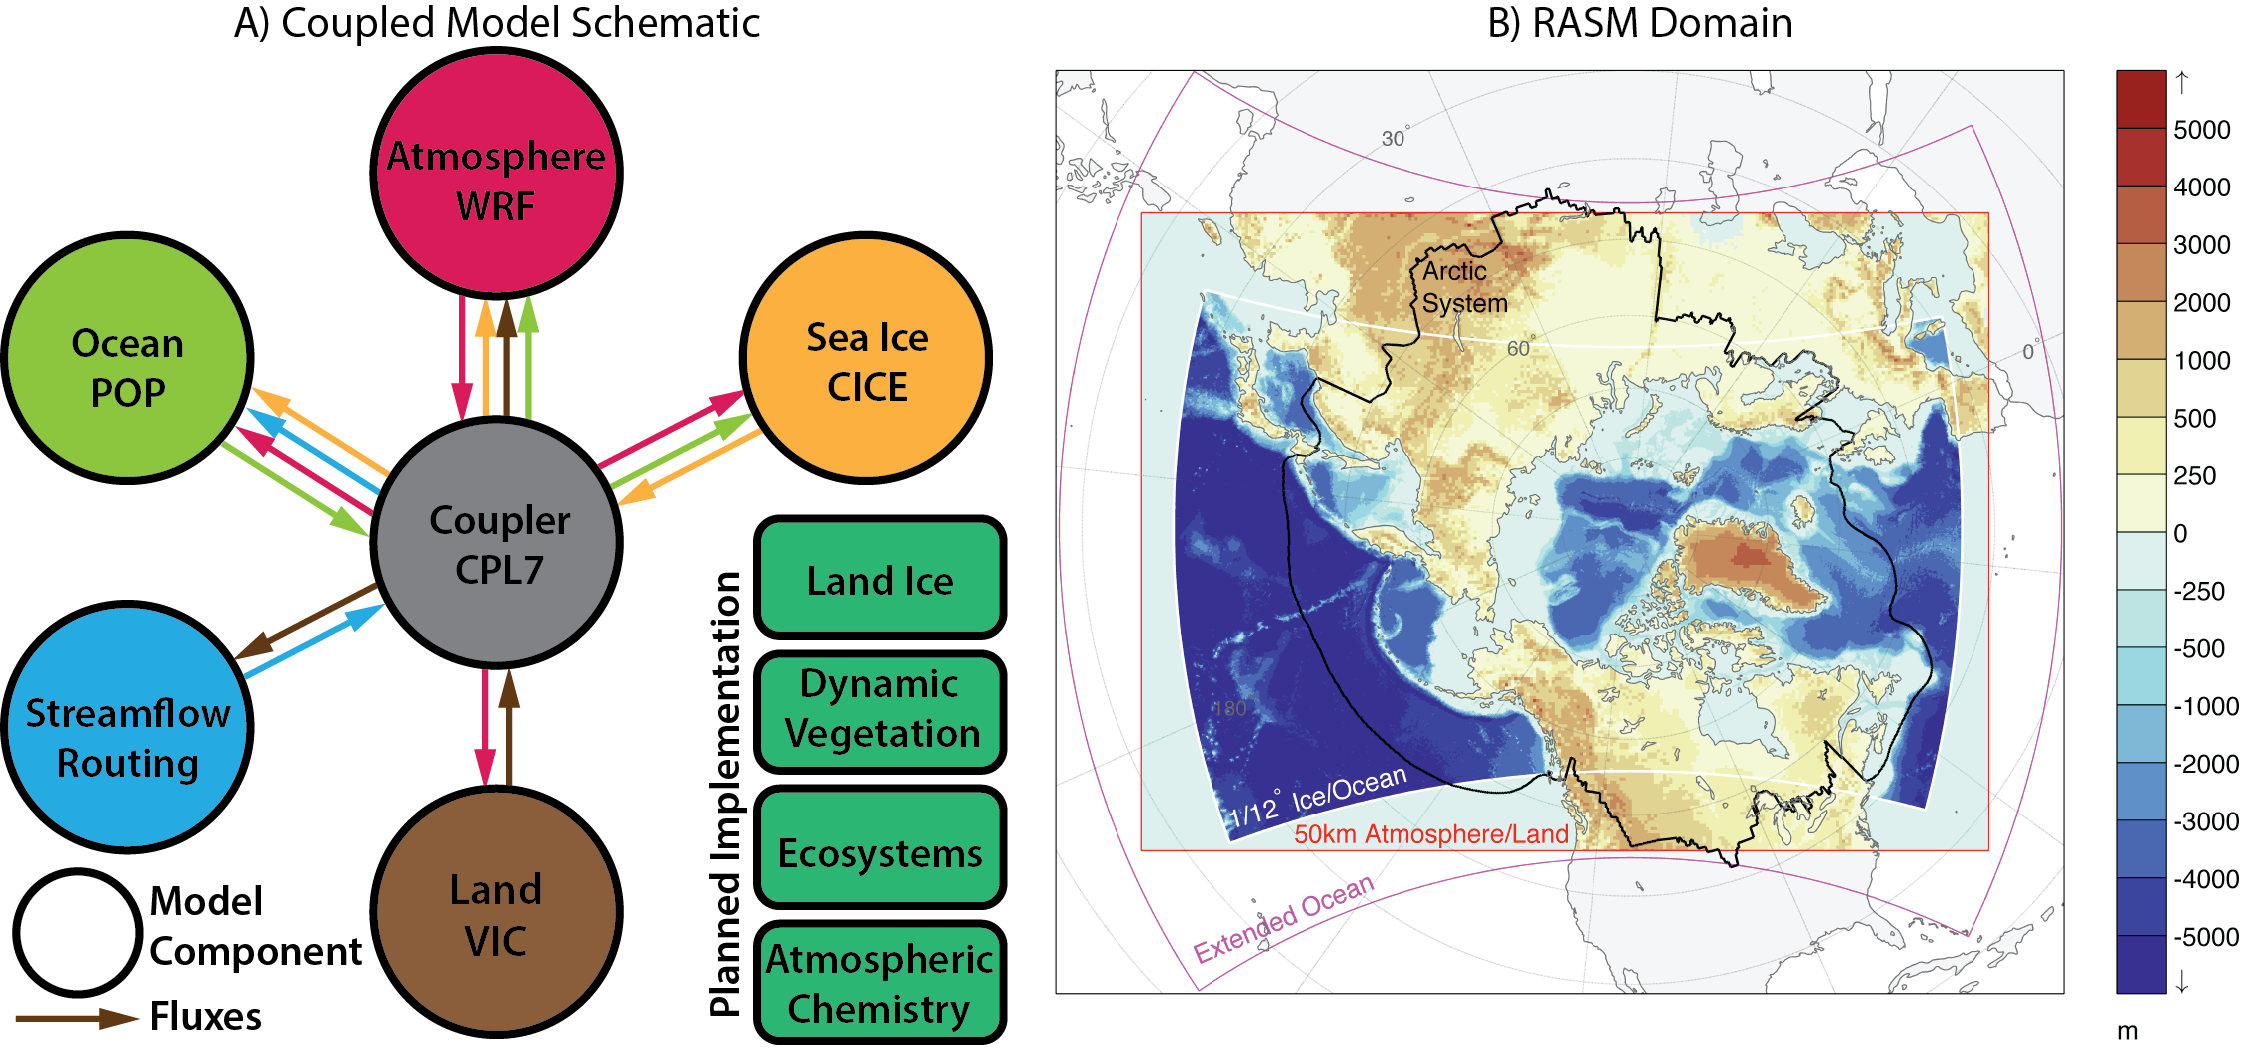
\includegraphics[width=40pc,natwidth=1]{Figure_1}
\caption{RASM domain showing river and ocean basins.}
\label{fig:1}
\end{figure}

\clearpage
\begin{figure}
\noindent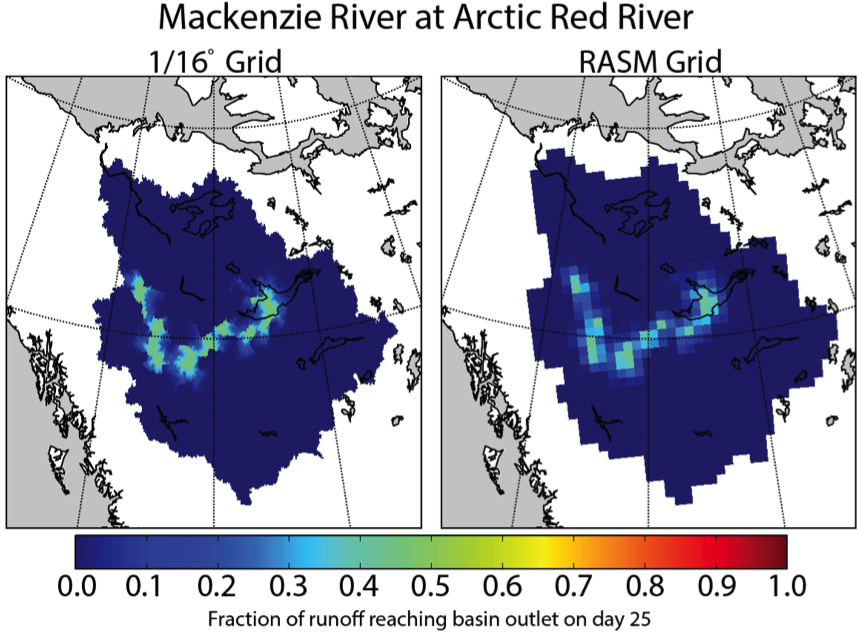
\includegraphics[width=40pc,natwidth=1]{Figure_2}
\caption{Example of a remapped unit hydrograph grid for outlet location of Mackenzie River at Arctic Red River. This figure depicts the fraction of runoff generated reaching the outlet point on day 25 for the 1/16th degree grid and the RASM 50-km grid.}
\label{fig:2}
\end{figure}

\clearpage
\begin{figure}
\noindent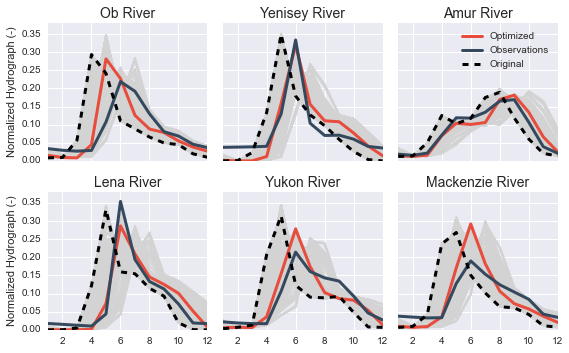
\includegraphics[width=40pc,natwidth=1]{Figure_3}
\caption{Normalized hydrographs for largest 6 river basins from.  Each trace (grey) represents a individaul calibration ensemble member. The observed (normalized) hydrograph for each basin is shown in blue and the hydrograph using the "Orignal" or "Fast" parameters is shown in dash-black.}
\label{fig:3}
\end{figure}

\clearpage
\begin{figure}
\noindent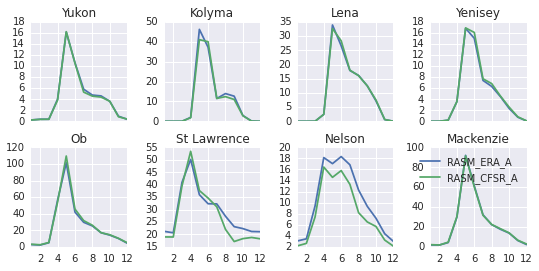
\includegraphics[width=40pc,natwidth=1]{Figure_4}
\caption{Composite parameter space performance}
\label{fig:4}
\end{figure}

\clearpage
\begin{figure}
\noindent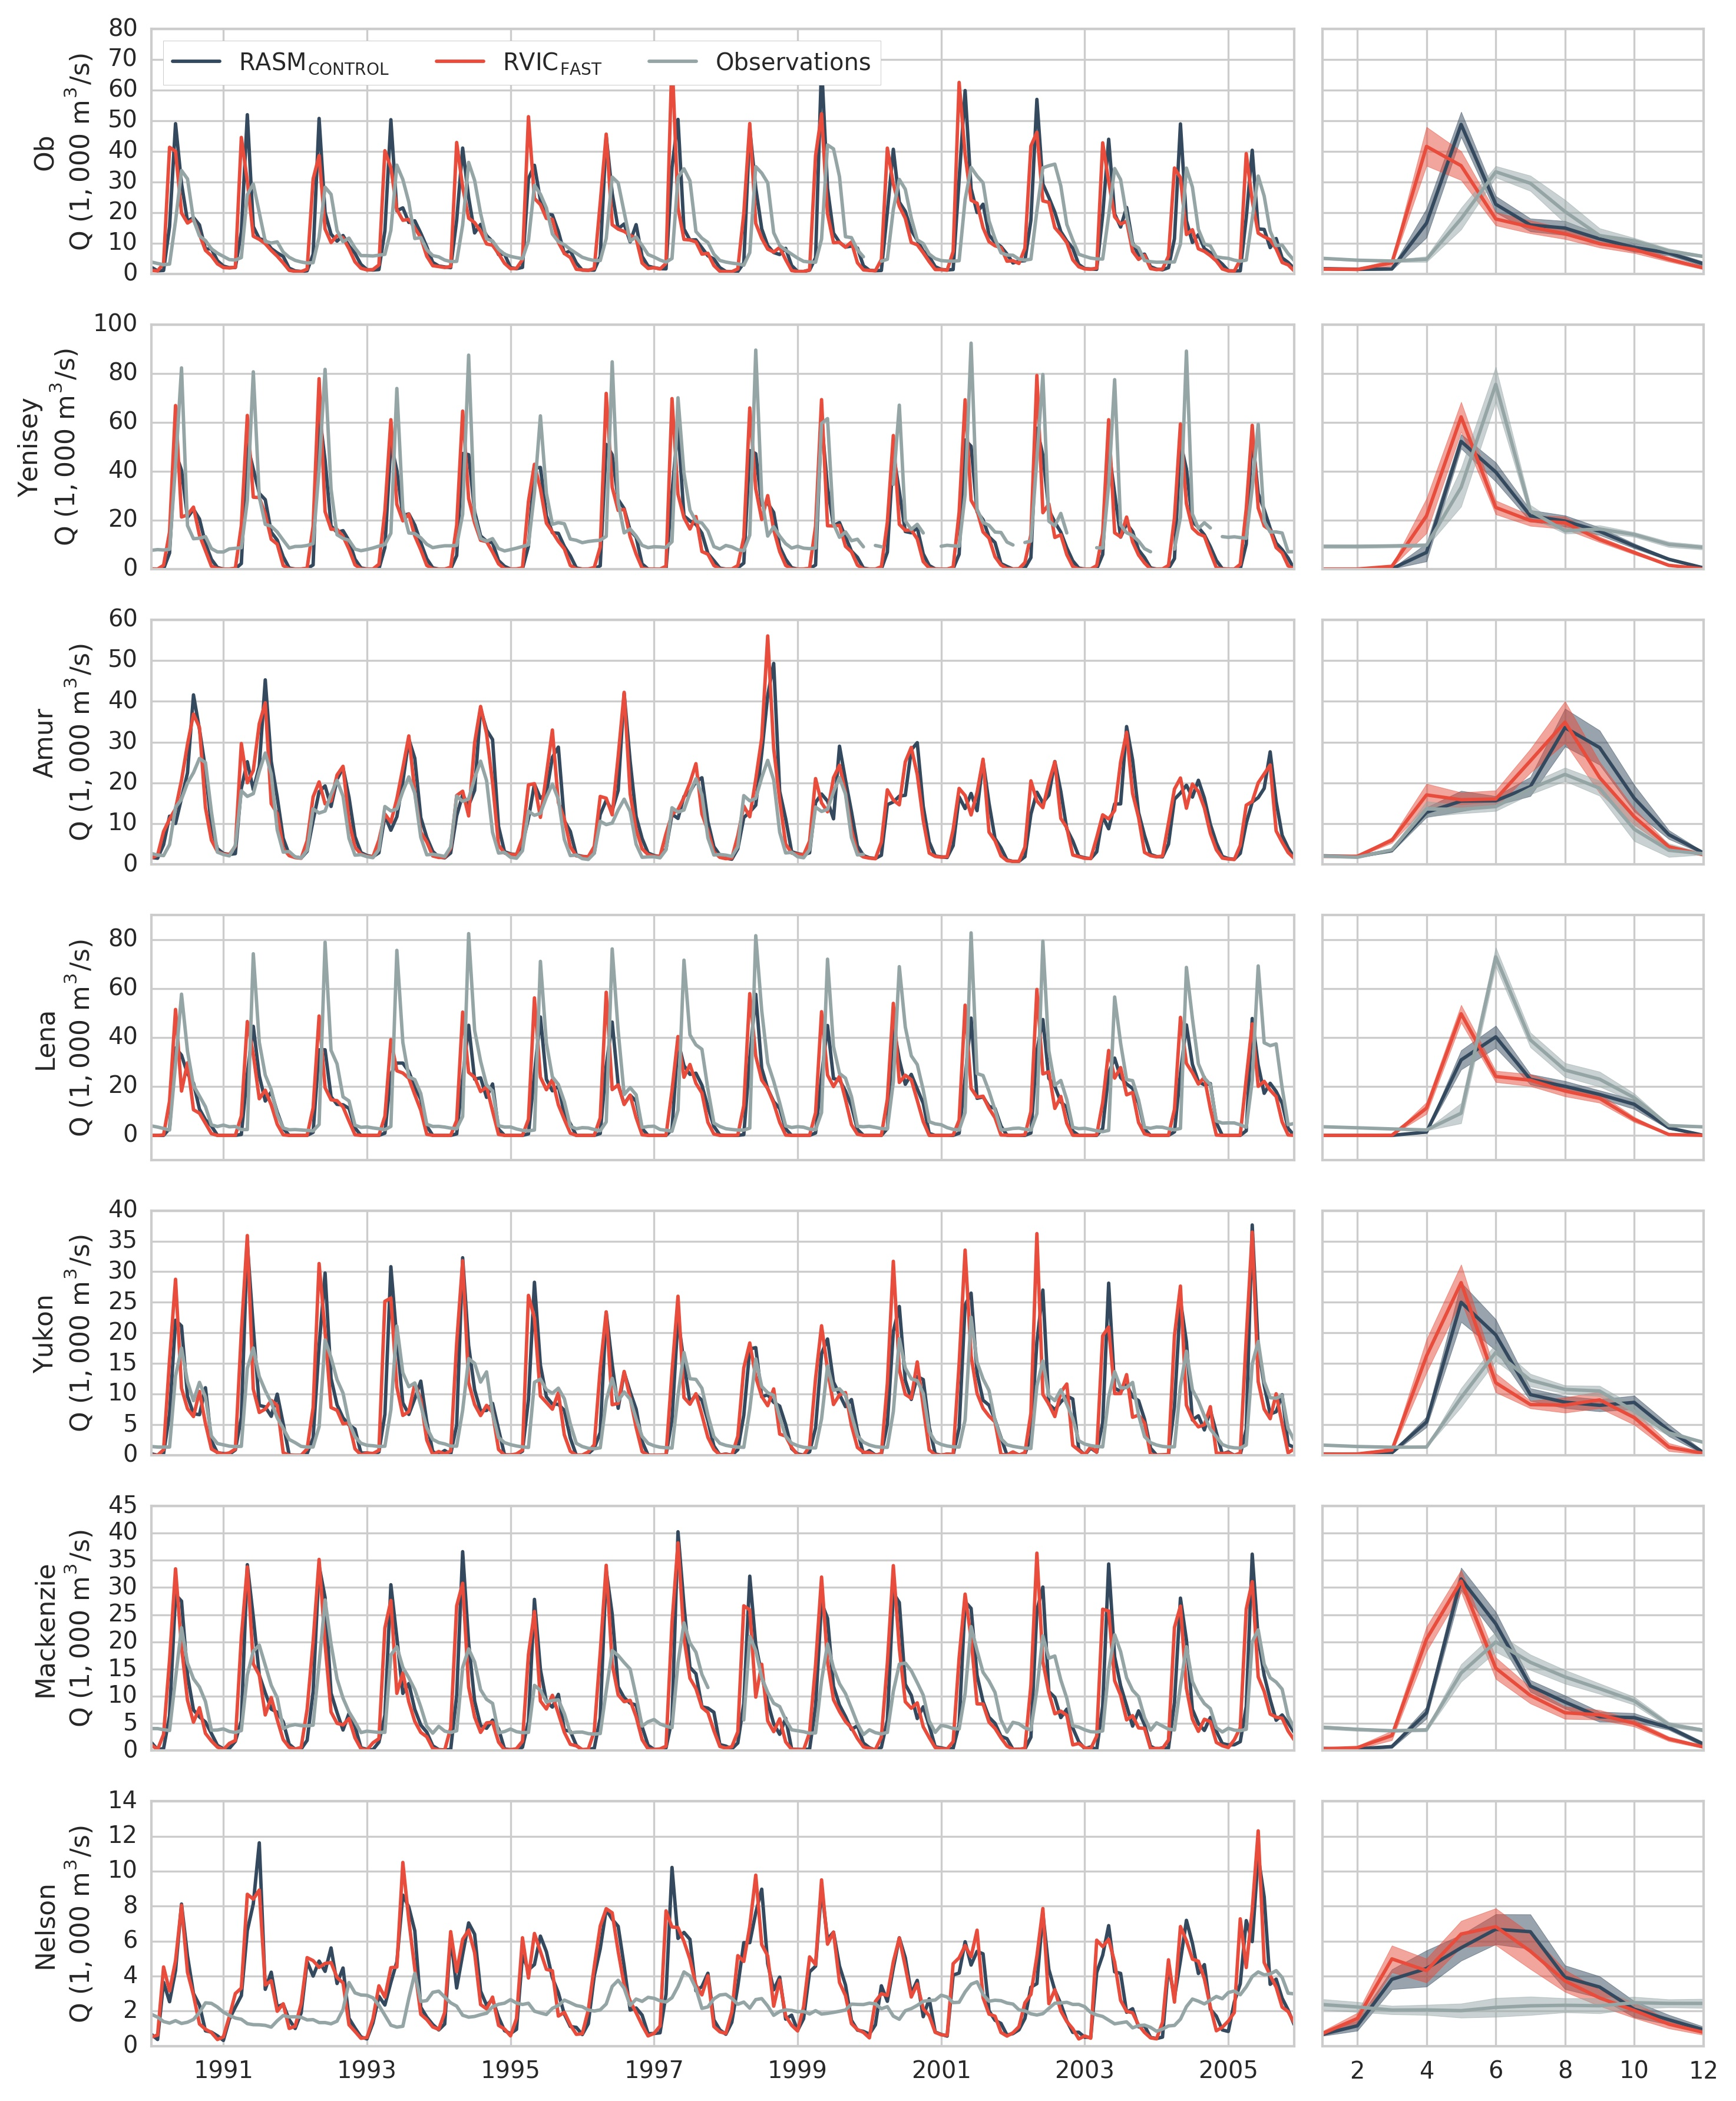
\includegraphics[width=40pc,natwidth=1]{Figure_5}
\caption{Routed hydrographs for largest 6 river basins compared to observations from \citet{Dai_2009}.}
\label{fig:5}
\end{figure}

\clearpage
\begin{figure}
\noindent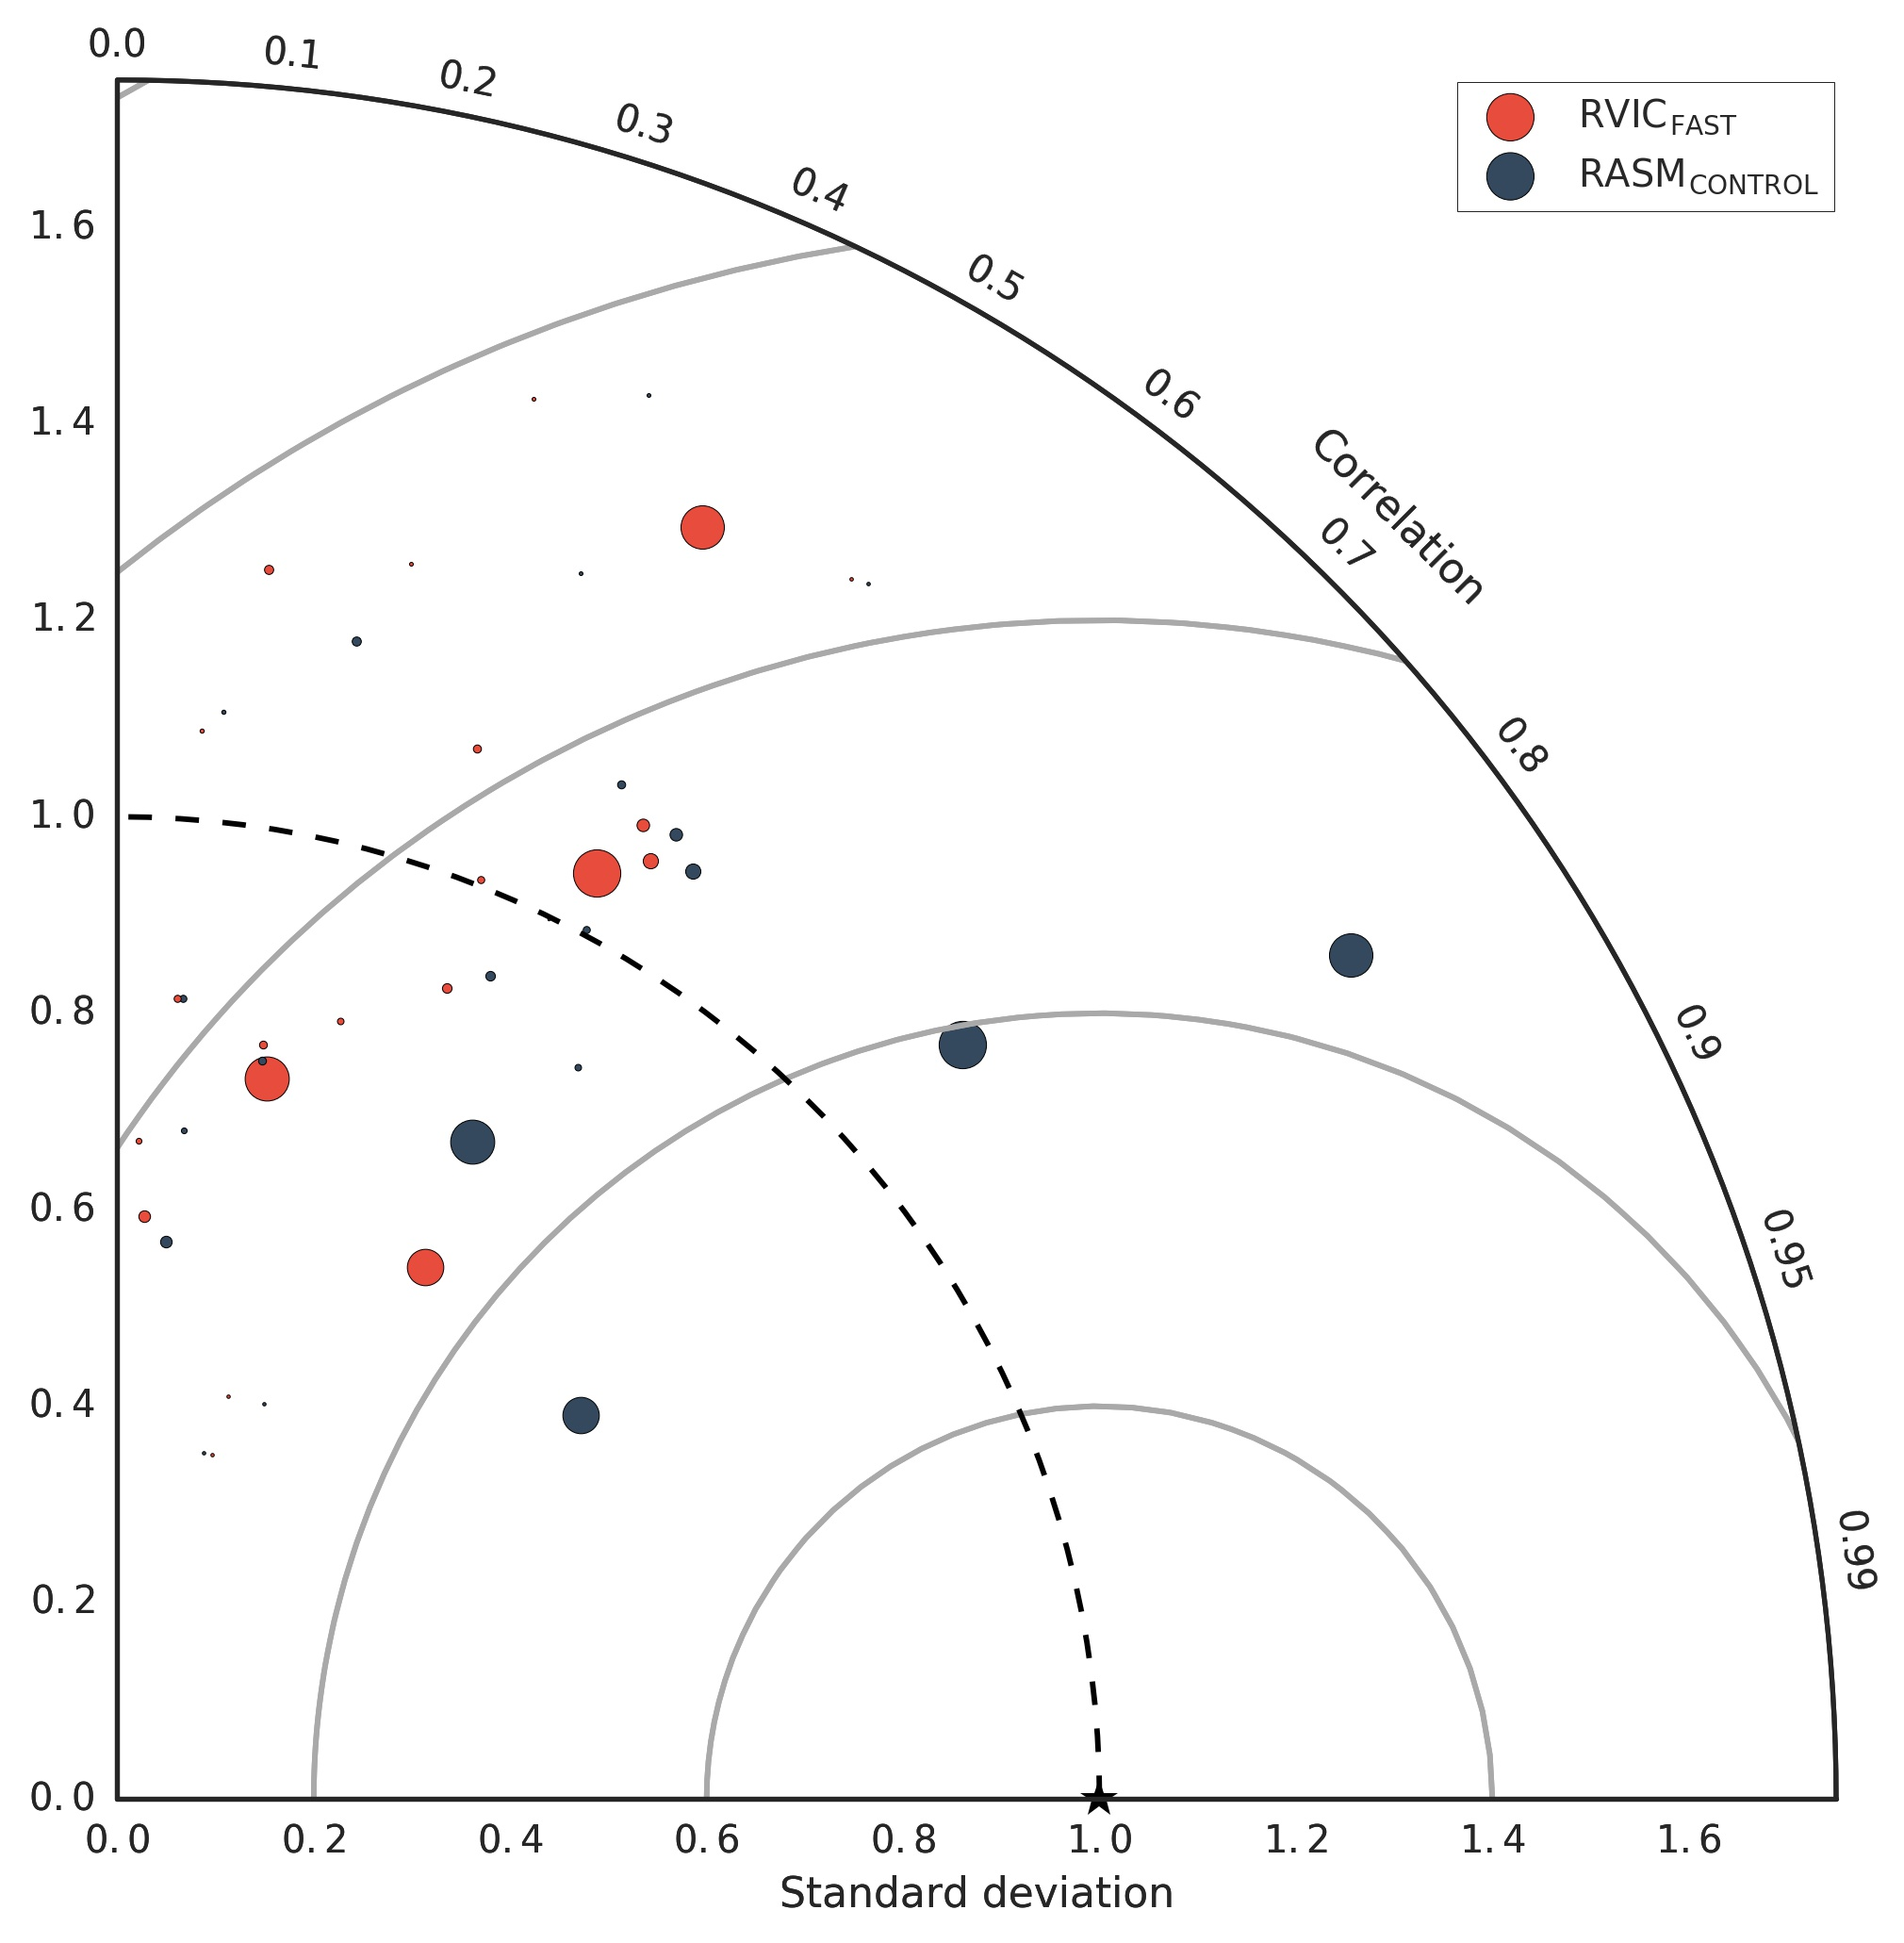
\includegraphics[width=40pc,natwidth=1]{Figure_6}
\caption{Taylor Diagram}
\label{fig:6}
\end{figure}

\clearpage
\begin{figure}
\noindent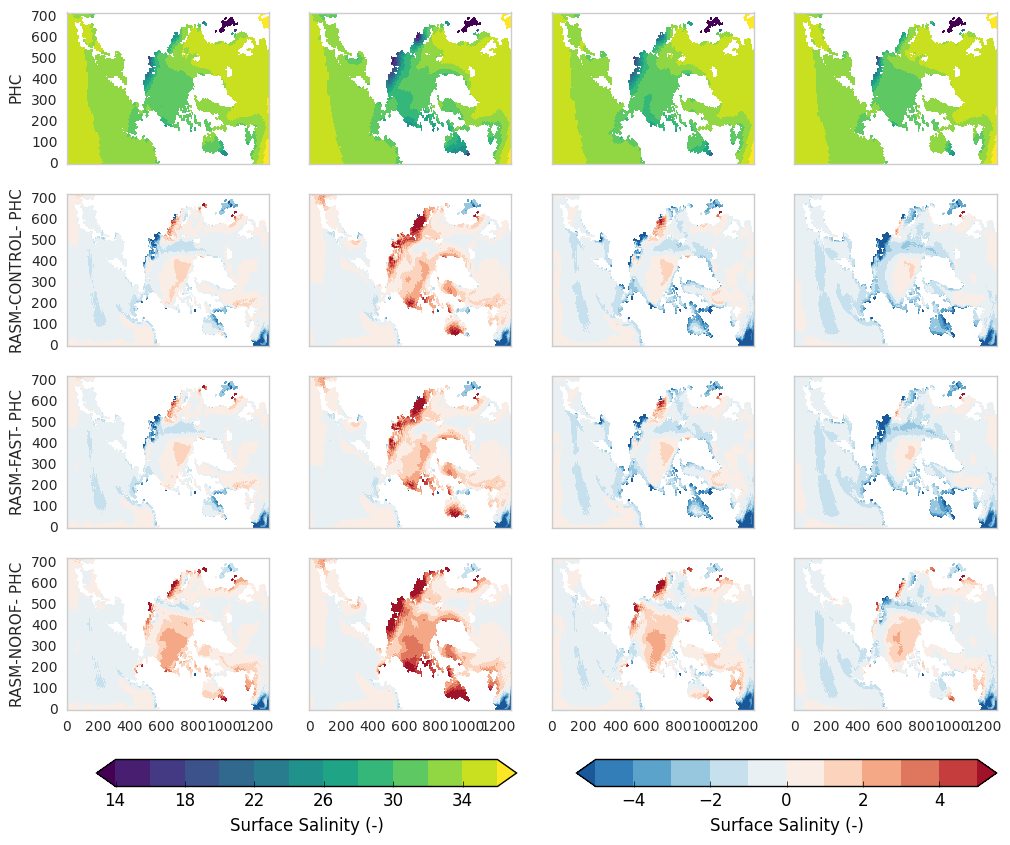
\includegraphics[width=40pc,natwidth=1]{Figure_7}
\caption{PLACEHOLDER: Seasonal mean surface ocean salinity for $RASM_{CONTROL}$, $RVIC_{FAST}$, and $RASM_{NOROF}$ compared to PHC climatology.}
\label{fig:7}
\end{figure}

\clearpage
\begin{figure}
\noindent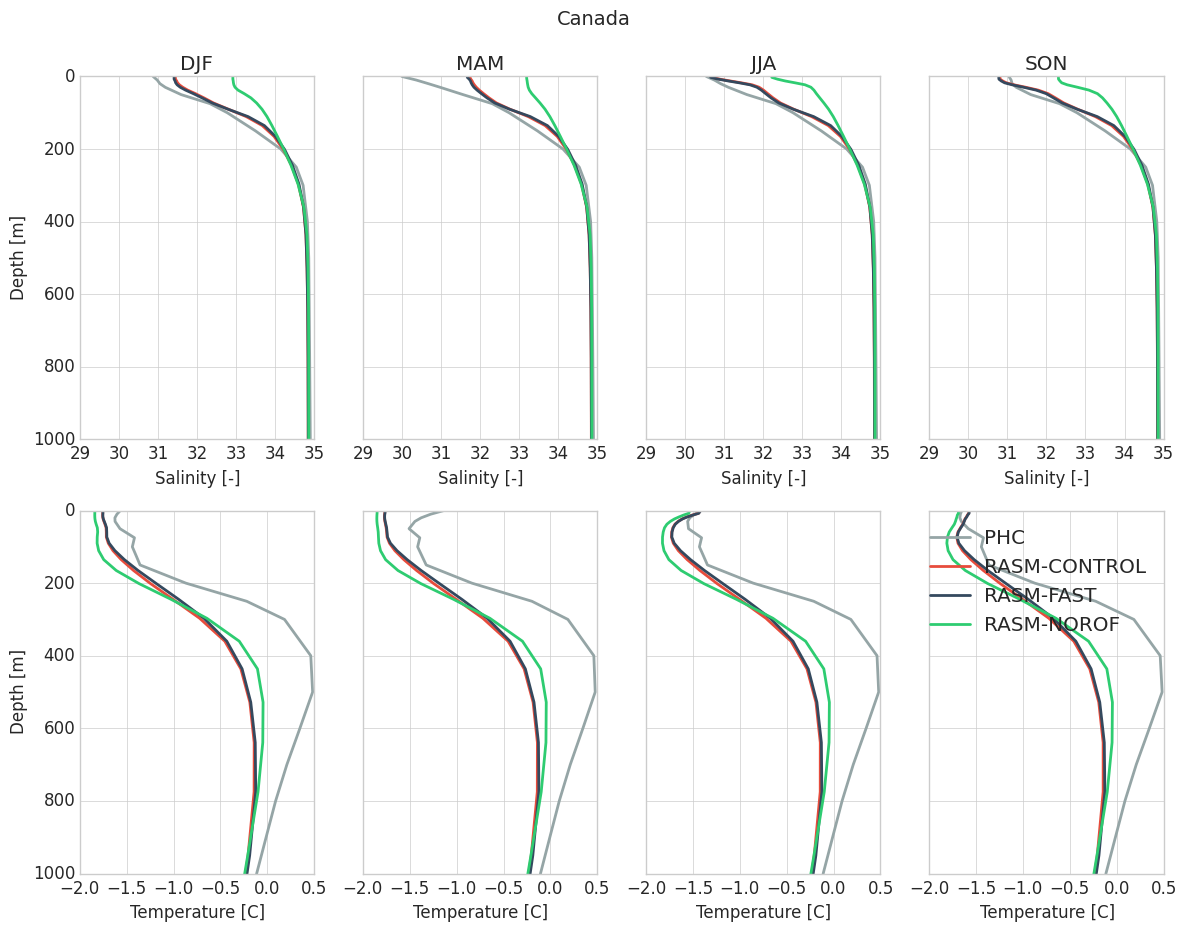
\includegraphics[width=40pc,natwidth=1]{Figure_8}
\caption{PLACEHOLDER: Seasonal mean ocean basin averaged depth prfiles of salinity and temperature for $RASM_{CONTROL}$, $RVIC_{FAST}$, and $RASM_{NOROF}$ compared to PHC climatology.}
\label{fig:8}
\end{figure}


%
% ---------------
% EXAMPLE TABLE
%
\clearpage

\begin{table}
\caption{Placeholder for table 1}
\centering
\begin{tabular}{l c}
\hline
Run  & Time (min)  \\
\hline
 $l1$  & 260   \\
 $l2$  & 300   \\
 $l3$  & 340   \\
 $h1$  & 270   \\
 $h2$  & 250   \\
 $h3$  & 380   \\
 $r1$  & 370   \\
 $r2$  & 390   \\
\hline
\end{tabular}
\tablenotetext{a}{Footnote text here.}
\label{table:1}
\end{table}

\clearpage

\begin{table}
\caption{Placeholder for table 2}
\centering
\begin{tabular}{l c}
\hline
Run  & Time (min)  \\
\hline
 $l1$  & 260   \\
 $l2$  & 300   \\
 $l3$  & 340   \\
 $h1$  & 270   \\
 $h2$  & 250   \\
 $h3$  & 380   \\
 $r1$  & 370   \\
 $r2$  & 390   \\
\hline
\end{tabular}
\tablenotetext{a}{Footnote text here.}
\label{table:2}
\end{table}

% See below for how to make sideways figures or tables.

\end{document}

%%%%%%%%%%%%%%%%%%%%%%%%%%%%%%%%%%%%%%%%%%%%%%%%%%%%%%%%%%%%%%%

More Information and Advice:

%% ------------------------------------------------------------------------ %%
%
%  SECTION HEADS
%
%% ------------------------------------------------------------------------ %%

% Capitalize the first letter of each word (except for
% prepositions, conjunctions, and articles that are
% three or fewer letters).

% AGU follows standard outline style; therefore, there cannot be a section 1 without
% a section 2, or a section 2.3.1 without a section 2.3.2.
% Please make sure your section numbers are balanced.
% ---------------
% Level 1 head
%
% Use the \section{} command to identify level 1 heads;
% type the appropriate head wording between the curly
% brackets, as shown below.
%
%An example:
%\section{Level 1 Head: Introduction}
%
% ---------------
% Level 2 head
%
% Use the \subsection{} command to identify level 2 heads.
%An example:
%\subsection{Level 2 Head}
%
% ---------------
% Level 3 head
%
% Use the \subsubsection{} command to identify level 3 heads
%An example:
%\subsubsection{Level 3 Head}
%
%---------------
% Level 4 head
%
% Use the \subsubsubsection{} command to identify level 3 heads
% An example:
%\subsubsubsection{Level 4 Head} An example.
%
%% ------------------------------------------------------------------------ %%
%
%  IN-TEXT LISTS
%
%% ------------------------------------------------------------------------ %%
%
% Do not use bulleted lists; enumerated lists are okay.
% \begin{enumerate}
% \item
% \item
% \item
% \end{enumerate}
%
%% ------------------------------------------------------------------------ %%
%
%  EQUATIONS
%
%% ------------------------------------------------------------------------ %%

% Single-line equations are centered.
% Equation arrays will appear left-aligned.

Math coded inside display math mode \[ ...\]
 will not be numbered, e.g.,:
 \[ x^2=y^2 + z^2\]

 Math coded inside \begin{equation} and \end{equation} will
 be automatically numbered, e.g.,:
 \begin{equation}
 x^2=y^2 + z^2
 \end{equation}

% IF YOU HAVE MULTI-LINE EQUATIONS, PLEASE
% BREAK THE EQUATIONS INTO TWO OR MORE LINES
% OF SINGLE COLUMN WIDTH (20 pc, 8.3 cm)
% using double backslashes (\\).

% To create multiline equations, use the
% \begin{eqnarray} and \end{eqnarray} environment
% as demonstrated below.
\begin{eqnarray}
  x_{1} & = & (x - x_{0}) \cos \Theta \nonumber \\
        && + (y - y_{0}) \sin \Theta  \nonumber \\
  y_{1} & = & -(x - x_{0}) \sin \Theta \nonumber \\
        && + (y - y_{0}) \cos \Theta.
\end{eqnarray}

%If you don't want an equation number, use the star form:
%\begin{eqnarray*}...\end{eqnarray*}

% Break each line at a sign of operation
% (+, -, etc.) if possible, with the sign of operation
% on the new line.

% Indent second and subsequent lines to align with
% the first character following the equal sign on the
% first line.

% Use an \hspace{} command to insert horizontal space
% into your equation if necessary. Place an appropriate
% unit of measure between the curly braces, e.g.
% \hspace{1in}; you may have to experiment to achieve
% the correct amount of space.


%% ------------------------------------------------------------------------ %%
%
%  EQUATION NUMBERING: COUNTER
%
%% ------------------------------------------------------------------------ %%

% You may change equation numbering by resetting
% the equation counter or by explicitly numbering
% an equation.

% To explicitly number an equation, type \eqnum{}
% (with the desired number between the brackets)
% after the \begin{equation} or \begin{eqnarray}
% command.  The \eqnum{} command will affect only
% the equation it appears with; LaTeX will number
% any equations appearing later in the manuscript
% according to the equation counter.
%

% If you have a multiline equation that needs only
% one equation number, use a \nonumber command in
% front of the double backslashes (\\) as shown in
% the multiline equation above.

%% ------------------------------------------------------------------------ %%
%
%  SIDEWAYS FIGURE AND TABLE EXAMPLES
%
%% ------------------------------------------------------------------------ %%
%
% For tables and figures, add \usepackage{rotating} to the paper and add the rotating.sty file to the folder.
% AGU prefers the use of {sidewaystable} over {landscapetable} as it causes fewer problems.
%
% \begin{sidewaysfigure}
% \includegraphics[width=20pc]{samplefigure.eps}
% \caption{caption here}
% \label{label_here}
% \end{sidewaysfigure}
%
%
%
% \begin{sidewaystable}
% \caption{}
% \begin{tabular}
% Table layout here.
% \end{tabular}
% \end{sidewaystable}
%
%
